
% *************** LEd - dokument oparty na szablonie pracy magisterskiej ***************

\documentclass[12pt,apalike,a4paper,openright,oneside,makeidx]{memoir}
% *************** Definicje stylu dokumentu ***************

% *********************************************************************************
% W piku tym zdefiniowany jest wygl�d dokumentu.
% Zmiany tutaj nie s� konieczne o ile nie zamierzasz zmienia� wygl�du dokumentu.
% *********************************************************************************

% *************** Za�adowanie pakiet�w ***************




\usepackage{graphicx}
\usepackage{float}
\usepackage{epsfig}
\usepackage{amsmath}
\usepackage{amssymb}
\usepackage{amsthm}
\usepackage{booktabs}
\usepackage{stmaryrd}
\usepackage{url}
\usepackage{longtable}

\usepackage{polski}
%\usepackage{indentfirst}
\usepackage[cp1250]{inputenc}


\usepackage{listings}
\usepackage{amsmath}
\usepackage{amsfonts}
\usepackage{amssymb}
\usepackage{amsthm}
\usepackage{bookman}


%\renewcommand*{\lstlistingname}{Spis listing�w kodu}


%\renewcommand{\bf}{\textbf}












% *************** W��czenie tworzenia skorowidza ***************
\makeindex

% *************** Dodanie do pozycji bibliograficznych informacji o numerze strony, na kt�rej jest ona cytowana ***************
\usepackage{citeref}
\renewcommand{\bibitempages}[1]{\newblock {\scriptsize }}

% *************** Definicje niekt�rych kolor�w ***************
\usepackage{color}

\definecolor{greenyellow}   {cmyk}{0.15, 0   , 0.69, 0   }
\definecolor{yellow}        {cmyk}{0   , 0   , 1   , 0   }
\definecolor{goldenrod}     {cmyk}{0   , 0.10, 0.84, 0   }
\definecolor{dandelion}     {cmyk}{0   , 0.29, 0.84, 0   }
\definecolor{apricot}       {cmyk}{0   , 0.32, 0.52, 0   }
\definecolor{peach}         {cmyk}{0   , 0.50, 0.70, 0   }
\definecolor{melon}         {cmyk}{0   , 0.46, 0.50, 0   }
\definecolor{yelloworange}  {cmyk}{0   , 0.42, 1   , 0   }
\definecolor{orange}        {cmyk}{0   , 0.61, 0.87, 0   }
\definecolor{burntorange}   {cmyk}{0   , 0.51, 1   , 0   }
\definecolor{bittersweet}   {cmyk}{0   , 0.75, 1   , 0.24}
\definecolor{redorange}     {cmyk}{0   , 0.77, 0.87, 0   }
\definecolor{mahogany}      {cmyk}{0   , 0.85, 0.87, 0.35}
\definecolor{maroon}        {cmyk}{0   , 0.87, 0.68, 0.32}
\definecolor{brickred}      {cmyk}{0   , 0.89, 0.94, 0.28}
\definecolor{red}           {cmyk}{0   , 1   , 1   , 0   }
\definecolor{orangered}     {cmyk}{0   , 1   , 0.50, 0   }
\definecolor{rubinered}     {cmyk}{0   , 1   , 0.13, 0   }
\definecolor{wildstrawberry}{cmyk}{0   , 0.96, 0.39, 0   }
\definecolor{salmon}        {cmyk}{0   , 0.53, 0.38, 0   }
\definecolor{carnationpink} {cmyk}{0   , 0.63, 0   , 0   }
\definecolor{magenta}       {cmyk}{0   , 1   , 0   , 0   }
\definecolor{violetred}     {cmyk}{0   , 0.81, 0   , 0   }
\definecolor{rhodamine}     {cmyk}{0   , 0.82, 0   , 0   }
\definecolor{mulberry}      {cmyk}{0.34, 0.90, 0   , 0.02}
\definecolor{redviolet}     {cmyk}{0.07, 0.90, 0   , 0.34}
\definecolor{fuchsia}       {cmyk}{0.47, 0.91, 0   , 0.08}
\definecolor{lavender}      {cmyk}{0   , 0.48, 0   , 0   }
\definecolor{thistle}       {cmyk}{0.12, 0.59, 0   , 0   }
\definecolor{orchid}        {cmyk}{0.32, 0.64, 0   , 0   }
\definecolor{darkorchid}    {cmyk}{0.40, 0.80, 0.20, 0   }
\definecolor{purple}        {cmyk}{0.45, 0.86, 0   , 0   }
\definecolor{plum}          {cmyk}{0.50, 1   , 0   , 0   }
\definecolor{violet}        {cmyk}{0.79, 0.88, 0   , 0   }
\definecolor{royalpurple}   {cmyk}{0.75, 0.90, 0   , 0   }
\definecolor{blueviolet}    {cmyk}{0.86, 0.91, 0   , 0.04}
\definecolor{periwinkle}    {cmyk}{0.57, 0.55, 0   , 0   }
\definecolor{cadetblue}     {cmyk}{0.62, 0.57, 0.23, 0   }
\definecolor{cornflowerblue}{cmyk}{0.65, 0.13, 0   , 0   }
\definecolor{midnightblue}  {cmyk}{0.98, 0.13, 0   , 0.43}
\definecolor{navyblue}      {cmyk}{0.94, 0.54, 0   , 0   }
\definecolor{royalblue}     {cmyk}{1   , 0.50, 0   , 0   }
\definecolor{blue}          {cmyk}{1   , 1   , 0   , 0   }
\definecolor{cerulean}      {cmyk}{0.94, 0.11, 0   , 0   }
\definecolor{cyan}          {cmyk}{1   , 0   , 0   , 0   }
\definecolor{processblue}   {cmyk}{0.96, 0   , 0   , 0   }
\definecolor{skyblue}       {cmyk}{0.62, 0   , 0.12, 0   }
\definecolor{turquoise}     {cmyk}{0.85, 0   , 0.20, 0   }
\definecolor{tealblue}      {cmyk}{0.86, 0   , 0.34, 0.02}
\definecolor{aquamarine}    {cmyk}{0.82, 0   , 0.30, 0   }
\definecolor{bluegreen}     {cmyk}{0.85, 0   , 0.33, 0   }
\definecolor{emerald}       {cmyk}{1   , 0   , 0.50, 0   }
\definecolor{junglegreen}   {cmyk}{0.99, 0   , 0.52, 0   }
\definecolor{seagreen}      {cmyk}{0.69, 0   , 0.50, 0   }
\definecolor{green}         {cmyk}{1   , 0   , 1   , 0   }
\definecolor{forestgreen}   {cmyk}{0.91, 0   , 0.88, 0.12}
\definecolor{pinegreen}     {cmyk}{0.92, 0   , 0.59, 0.25}
\definecolor{limegreen}     {cmyk}{0.50, 0   , 1   , 0   }
\definecolor{yellowgreen}   {cmyk}{0.44, 0   , 0.74, 0   }
\definecolor{springgreen}   {cmyk}{0.26, 0   , 0.76, 0   }
\definecolor{olivegreen}    {cmyk}{0.64, 0   , 0.95, 0.40}
\definecolor{rawsienna}     {cmyk}{0   , 0.72, 1   , 0.45}
\definecolor{sepia}         {cmyk}{0   , 0.83, 1   , 0.70}
\definecolor{brown}         {cmyk}{0   , 0.81, 1   , 0.60}
\definecolor{tan}           {cmyk}{0.14, 0.42, 0.56, 0   }
\definecolor{gray}          {cmyk}{0   , 0   , 0   , 0.50}
\definecolor{black}         {cmyk}{0   , 0   , 0   , 1   }
\definecolor{white}         {cmyk}{0   , 0   , 0   , 0   } 

% *************** W��czenie hyperlink�w w dokumentach PDF ***************
\ifpdf
    \pdfcompresslevel=9
        \usepackage[plainpages=false,pdfpagelabels,bookmarksnumbered,%
        colorlinks=false,%
        linkcolor=sepia,%
        citecolor=sepia,%
        filecolor=maroon,%
        pagecolor=red,%
        urlcolor=sepia,%
        pdftex,%
        unicode]{hyperref} 
    \input supp-mis.tex
    \input supp-pdf.tex
    \pdfimageresolution=600
    \usepackage{thumbpdf} 
\else
    \usepackage{hyperref}
\fi

\usepackage{memhfixc}

% *************** Wygl�d strony marginesy ***************
\settypeblocksize{*}{32pc}{1.618}
%Rozne marginesy
%\textwidth=16cm
%\setlrmargins{*}{20mm}{*}
%\setulmargins{*}{*}{1.3}

%Takie same
\setlrmargins{*}{1.47in}{*}
\setulmargins{*}{*}{1.3}

\setheadfoot{\onelineskip}{2\onelineskip}
\setheaderspaces{*}{2\onelineskip}{*}

\def\baselinestretch{1.1}

\checkandfixthelayout


% *************** Stylu rozdzia��w i podrozdzia��w ***************
\makechapterstyle{mychapterstyle}{%
    \renewcommand{\chapnamefont}{\LARGE\sffamily\bfseries}%
    \renewcommand{\chapnumfont}{\LARGE\sffamily\bfseries}%
    \renewcommand{\chaptitlefont}{\Huge\sffamily\bfseries}%
    \renewcommand{\printchaptertitle}[1]{%
        \chaptitlefont\hrule height 0.5pt \vspace{1em}%
        {##1}\vspace{1em}\hrule height 0.5pt%
        }%
    \renewcommand{\printchapternum}{%
        \chapnumfont\thechapter%
        }%
}

\chapterstyle{mychapterstyle}

\setsecheadstyle{\Large\sffamily\bfseries}
\setsubsecheadstyle{\large\sffamily\bfseries}
\setsubsubsecheadstyle{\normalfont\sffamily\bfseries}
\setparaheadstyle{\normalfont\sffamily}

\makeevenhead{headings}{\thepage}{}{\small\slshape\leftmark}
\makeoddhead{headings}{\small\slshape\rightmark}{}{\thepage}

% *************** Styl spisu tre�ci ***************
\settocdepth{subsection}

\setsecnumdepth{subsection}
\maxsecnumdepth{subsection}
\settocdepth{subsection}
\maxtocdepth{subsection}

% ********** Polecenia do mott **********
\setlength{\epigraphwidth}{0.57\textwidth}
\setlength{\epigraphrule}{0pt}
\setlength{\beforeepigraphskip}{1\baselineskip}
\setlength{\afterepigraphskip}{2\baselineskip}

\newcommand{\epitext}{\sffamily\itshape}
\newcommand{\epiauthor}{\sffamily\scshape ---~}
\newcommand{\epititle}{\sffamily\itshape}
\newcommand{\epidate}{\sffamily\scshape}
\newcommand{\episkip}{\medskip}

\newcommand{\myepigraph}[4]{%
	\epigraph{\epitext #1\episkip}{\epiauthor #2\\\epititle #3 \epidate(#4)}\noindent}

% *************** Inne ***************
\renewcommand{\thefootnote}{\fnsymbol{footnote}}

\DeclareGraphicsExtensions{.png, .bb}


% *************** Koniec definicji stylu dokumentu ***************



\begin{document}
% *************** Front matter ***************
\frontmatter
% *************** Front matter ***************

% ************************************************************
% W tym miejscu mo�esz zdefiniowa� wygl�d strony tytu�owej
% Mo�esz tak�e zdefiniowa� dedykacj� albo wy��czy� j�
% ************************************************************

% *************** Strona tytu�owa ***************
\pagestyle{empty}
\sffamily

\linespread{1.0}
\noindent

% \begin{figure}
%	\centering
%		
\includegraphics[width=1.0\textwidth]{logo.pdf}
%	\label{fig:logo}
% \end{figure}

\vfill\vfill
\begin{center}
    \Large\bfseries
    PRACA DYPLOMOWA - IN�YNIERSKA\\
\end{center}

\vfill
\begin{center}
    \Large
    Konrad Rodzik\\
    nr albumu: 215039
\end{center}

\vfill
\begin{center}
    \Large\bfseries
    NVIDIA CUDA jako technologia przy�pieszaj�ca metode �ledzenia promieni
\end{center}

\vfill\vfill\vfill
\begin{flushright}
    \Large
    Kierownik pracy:\\ Prof. nazw. dr hab. in�. Dariusz Sawicki
\end{flushright}
\vfill

\begin{flushleft}
....................................................\\
\ \ ocena pracy \\
\vfill
....................................................\\
\ \ data i podpis Przewodnicz�cego\\
\ \ Komisji Egzaminacyjnej Dyplomowego
\end{flushleft}

\vfill
\begin{center}
\large
    Warszawa, 2011
\end{center}


\chapter*{�yciorys}
Urodzi�em si�  1 listopada 1987 r.  w Radomiu w rodzinie inteligenckiej. Ojciec in�ynier, matka z wykszta�cenia prawnik.
W roku 2003 uko�czy�em gimnazjum i rozpocz��em nauk� w VI Liceum Og�lnokszta�c�cym im. J. Kochanowskiego w Radomiu w klasie o profilu matematyczno-fizyczno-informatycznym. 
Po maturze w roku 2006 zosta�em studentem na Wydziale Elektroniki i Technik Informacyjnych Politechniki Warszawskiej na kierunku Telekomunikacja.  

Od 2008 r. jestem cz�onkiem ko�a naukowego  "Brama". Zajmuj� si� badaniami i rozwojem system�w i aplikacji mobilnych. 
Interesuj� si� systemami oraz aplikacjami mobilnymi oraz mechanizmami wspierania proces�w nauki i zapami�tywania. 

Moje zainteresowania to: bieganie, sporty walki oraz windsurfing.

\cleardoublepage

\begin{abstract}
\noindent \textbf{Tytu�:  Mobilny system dobierania kierowc�w i pasa�er�w do wsp�lnej podr�y: "mobiStopowicz"}\\
Niniejsza praca in�ynierska opisuje projekt mobilnego systemu przeznaczonego dla kierowc�w i podr�nych, kt�rego celem jest wspieranie procesu dobierania si� do wsp�lnej podr�y. W pracy przeprowadzi�em wst�pn� analiz� sytuacji na rynku, opracowa�em algorytm parowania oraz zaprojektowa�em architektur� systemu. Nast�pnie zosta� opisany projekt, implementacja oraz perspektywa wdro�enia systemu.\\\\\\


\begin{center}\textbf{Abstract}\end{center}
\textbf{Title: Mobile system designed for pairing divers and travelers to collective travel: "mobiStopowicz"}\\
The bachelor thesis describes the mobile system aimed at pairing drivers and travelers to collective travel. In the thesis I have analyzed state of the art. Then pairing algorithm and architecture of the system was designed. The thesis also describes project, implementation and deployment opportunities of the mobiStopowicz system.

\end{abstract}

\clearpage

\rmfamily
\normalfont
% *************** Spis tre�ci ***************
\pagenumbering{roman}
\pagestyle{headings}
\tableofcontents

% *************** Koniec front matter ***************




\definecolor{ListingBackground}{rgb}{0.95,0.95,0.95}


\lstdefinestyle{outcode}
{
basicstyle={\footnotesize},
keywordstyle=\color[rgb]{0,0,1}, 
commentstyle=\color[rgb]{0.133,0.545,0.133}, 
stringstyle=\color[rgb]{0.627,0.126,0.941}, 
numbers=left, 
stepnumber=1, 
firstnumber=1,
numberfirstline=true,
numberblanklines=false, 
numbersep=10pt, 
tabsize=2,
xleftmargin=17pt,
framexleftmargin=3pt,
framexbottommargin=2pt,
framextopmargin=2pt,
framexrightmargin=0pt,
showstringspaces=true,
backgroundcolor={\color{ListingBackground}},
extendedchars=true,
% title=\lstname,
captionpos=b,
% abovecaptionskip=1pt,
% belowcaptionskip=1pt,
frame=tb,
framerule=0.1pt, 
}







% *************** Main matter ***************
\mainmatter
% ********** Podzi�kowania **********
\clearpage
\chapter*{Podzi�kowania}
Chcia�bym bardzo podzi�kowa� mojemu promotorowi za opiek� naukow� oraz cenne rady podczas pisania tej pracy.\\

Dodatkowo bardzo dzi�kuj� moim rodzicom oraz mojej dziewczynie. Bez ich wsparcia i bod�c�w motywacyjnych powstanie tej pracy nie by�o by mo�liwe.\\

Na ko�cu lecz nie mniej wa�ne podziekowania dla mojego sprz�tu, kt�ry du�o wycierpia� podczas powstawania niniejszej pracy. Karta graficzna wymieniana byla trzy razy...
 

% ********** Koniec podzi�kowa� **********

% ********** Rozdzia� 1 **********
\chapter{Wst�p}
\label{sec:chapter1}


\section{Wprowadzenie}
\label{sec:chapter1:Wprowadzenie}
Raytracing jest technik� s�u��c� do generowania foto realistycznych obraz�w scen 3D. Na przestrzeni lat technika ta ci�gle si� rozwija�a. Doczeka�a si� wielu modyfikacji, kt�re usprawniaj� proces generowania realistycznej grafiki. Takimi technikami mog� by� mi�dzy innymi PathTracing, PhotonMapping, Radiostity i wiele innych. Z dnia na dzie� wykorzystywanie raytracingu ci�gle ro�nie. 
W dzisiejszych czasach w grafice komputerowej oraz w kinematografii do uzyskania realistycznych efekt�w u�ywana jest metoda �ledzenia promieni. Dzi�ki takim zabiegom jeste�my w stanie dos�ownie zasymulowa� sceny oraz zjawiska, kt�re nie musz� istnie� w rzeczywistym �wiecie. Czas generowania pojedynczej klatki/uj�cia takiej sceny niekiedy potrafi by� liczony nawet w godzinach. Dlatego technika ta nie doczeka�a si� jeszcze swojej wielkiej chwili w przemy�le rozrywkowym jakim s� np. gry komputerowe oraz inne aplikacje generuj�ce grafik� 3D w czasie rzeczywistym.

\begin{figure}[h]
\begin{center}
\begin{minipage}[b]{4cm}
\centering
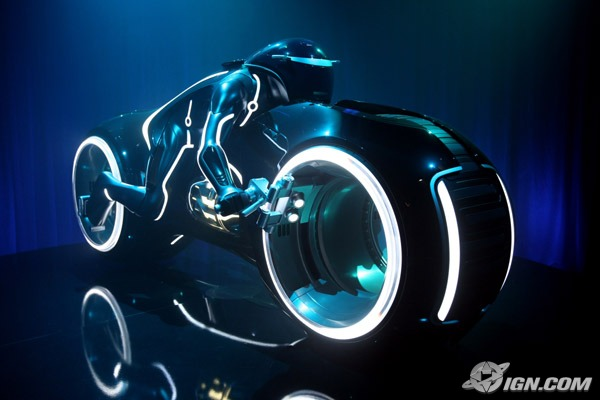
\includegraphics[width=\textwidth]{roz1/img/tron.jpg}\\\textit{a) Tron Legacy}
\end{minipage}
\begin{minipage}[b]{4cm}
\centering

\includegraphics[width=\textwidth]{roz1/img/avatar.jpg}\\\textit{b) Avatar}
\end{minipage}
\begin{minipage}[b]{4cm}
\centering

\includegraphics[width=\textwidth]{roz1/img/shreck.jpg}\\\textit{c) Shrek}
\end{minipage}
\caption{Uj�cia filmowe stworzone za pomoc� technik komputerowych}
\label{fig:filmy_rt}
\end{center}
\end{figure}


\section{Motywacja}
\label{sec:chapter1:Motywacja}
G��wnym bod�cem motywacyjnym do napisania tej pracy by�a ch�� poszerzenia dotychczasowej wiedzy na temat  przy�pieszania oblicze� przy pomocy nowej technologii NVIDIA CUDA. Dodatkowymi czynnikami motywacyjnymi by�o zami�owanie do grafiki komputerowej oraz do tworzenia aplikacji oblicze� czasu rzeczywistego. Na co dzie� zajmuj� si� programowaniem gier/aplikacji na komputery klasy PC oraz urz�dzenia mobilne. Uwa�am, �e w przysz�o�ci przedstawiona przeze mnie w tej pracy metoda �ledzenia promieni b�dzie mia�a zastosowanie w grach oraz aplikacjach wykorzystuj�cych grafik� czasu rzeczywistego.


\section{Terminologia wykorzystywana w pracy}
\label{sec:chapter1:terminologia}
\begin{itemize} 
\item Developer - Tw�rca/programista aplikacji
\item CUDA - Technologia stworzona przez firm� NVIDIA w 2007 roku. Umo�liwia r�wnoleg�e obliczenia na mikroprocesorach karty graficznej
\item Raytracing - metoda generowania obrazu za pomoc� �ledzenia promieni.
\item Benchmark - Aplikacji testowa, kt�ra profiluje wydajno�� i zbiera informacje.
\item Warp - blok w�tk�w przydzielony na multiprocesor
\item DirectX - technologia graficzna firmy Microsoft. Umo�liwia wy�wietlanie wysokiej jako�ci grafiki 2D/3D.
\item Aliasing - Zdeformowany, o z�ej jako�ci obraz kt�ry powstaje podczas rastaryzacji, powodowany przez zbyt ma�a cz�stotliwo�� pr�bkowania na pojedy�czy pixel obrazu. Przeciwdzia�a si� temu efektowi poprzez antyaliasing oraz w raytracingu poprzez super-sampling
\item Super-sampling - spos�b na zwi�kszenie jako�ci generowanych scen. Polega na �ledzeniu wielu promieni �wietlnych na pojedy�czy pixel generowanego obrazu.
\end{itemize} 


\section{Dost�pne technologie, pozwalaj�ce zr�wnolegli� obliczenia na kartach graficznych}
\label{sec:chapter1:Dost�pneTechnologie}
Poni�ej zaprez�towane zosta�y trzy wybrane technologi� wspomagaj�ce r�wnoleg�e  obliczenia na kartach graficznych. Niemniej jednak badania przeprowadzone i opisane w dalszej cz�ci pracy b�d� skupia�y si� na wykorzystaniu jednej z tych metod, a mianowicie technologii NVIDIA CUDA.


\subsection{Open Computing Language (OpenCL)}
Technologia tak zainicjowana zosta�a przez firm� Apple. Do inicjatywy i rozwijania tej technologii w��czy�y si� w p�niejszym czasie inne firmy takie jak: AMD, IBM, Intel, NVIDIA. W roku 2008 sformowana zosta�a grupa Khronos skupiaj�ca powy�sze firmy oraz wiele innych nale��cych do bran�y IT. Grupa ta czuwa nad rozwojem technologii OpenCL. 
Technologia tak pozwala na pisanie kodu kt�ry jest przeno�ny mi�dzy wieloma platformami: komputery, urz�dzenia przeno�ne, klastry obliczeniowe. OpenCL pozwala rozprasza� obliczenia na jednostki procesorowe CPU oraz na architektury graficzne GPU. Bardzo wa�n� zalet� OpenCL jest to, �e pisanie z u�yciem tej technologii nie jest zale�ne od sprz�tu na jakim b�dzie ona uruchamiana.

\subsection{ATI Stream Computing}
Technologia ta zosta�a stworzona przez firm� AMD. Za pomoc� tej platformy jeste�my w stanie przeprowadza� z�o�one obliczenia na sprz�cie produkowanym przez AMD.
W sk��d ca�ego pakietu ATI Stream Computing wchodzi autorski j�zyk ATI Brook+ i kompilator tego� j�zyka. Dodatkowo ATI wspiera developer�w w�asn� biblioteka matematyczna (AMD Core Math Library) oraz narz�dziami do profilowania wydajno�ci kodu (Strem Kernel Analyzer). Technologia ATI konkuruje od dawna z technologi� NVIDIA CUDA.


\subsection{NVIDIA CUDA}
CUDA (Compute Unified Device Architecture) jest technologia opracowan� przez firm� NVIDIA. Swoje pocz�tki CUDA mia�a w 2007 roku i do dzi� jest wiod�c� technologi� strumieniowego przetwarzania danych z wykorzystaniem uk�ad�w graficznych GPU. Dalszemu opisu niniejszej technologii po�wi�cony zostanie osobny rozdzia�.

\begin{figure}[h]
\begin{center}
\begin{minipage}[b]{4cm}
\centering

\includegraphics[width=\textwidth]{roz1/img/cuda_logo.jpg}\\\textit{a) Logo NVIDIA CUDA}
\end{minipage}
\begin{minipage}[b]{4cm}
\centering

\includegraphics[width=\textwidth]{roz1/img/ati_logo.jpg}\\\textit{b) Logo ATI Stream Computing}
\end{minipage}
\caption{Loga dw�ch konkurencyjnych ze sob� technologii przetwarzania r�wnoleg�ego na kartach graficznych}
\label{fig:cuda_ati}
\end{center}
\end{figure}


\clearpage

% ********** Rozdzia� 2 **********
\chapter{Cele pracy}
\label{sec:chapter2}


\section{Opracowanie techniki zr�wnoleglenia i przyspieszenia metody �ledzenia promieni przy u�yciu NVIDIA CUDA}
Celem niniejszej pracy jest przeniesienie a zarazem zr�wnoleglenie algorytmu �ledzenia promieni na procesory graficzne (GPU) firmy NVIDIA. Celem tak�e jest przy�pieszenie oblicze� standardowego wstecznego Raytracingu w celu jak najszybszego generowania obraz�w scen 3D.


\section{Projekt uniwersalnej aplikacji - benchmark}
W ramach projektu napisany zosta� uniwersalny system Raytracingu dzia�aj�cy na wielo rdzeniowych procesorach komputerowych (CPU), a tak�e na kartach graficznych (GPU) firmy NVIDIA kt�re obs�uguj� technologie NVIDIA CUDA. Aplikacja testowa jest benchmarkiem, kt�ry jest w stanie przetestowa� zadane sceny 3D na wielu r�nych konfiguracjach sprz�towych. Aplikacja ma za zadanie po uruchomieniu na komputerze u�ytkownika, testowa� wszelkie sceny z odpowiedniego katalogu. Dodatkowo zbiera� potrzebne informacje o sprz�cie u�ytkownika oraz czasy generowania obraz�w z ka�dej ze scen. Po przeprowadzeniu wszelkich test�w aplikacja jest w stanie wysla� na adres e-mail developera (w tym przypadku autora pracy) wszelkie zgromadzone dane.

% ********** Rozdzia� 3 **********
\chapter{Wprowadzenie do Raytracingu}
\label{sec:chapter3}


\section{Wst�pny opis}
\label{sec:chapter3:Wstep}
W rzeczywistym �wiecie promienie �wietlne rozchodz� si� od �r�d�a �wiat�a do obiekt�w znajduj�cych si� w �wiecie. Ka�de �r�d�o �wiat�a wysy�a niesko�czon� liczb� swoich promieni �wietlnych. Nast�pnie te promienie odbijaj�c si� od obiekt�w i trafiaj� do oczu obserwatora powoduj�c �e widzi on okre�lony kolor danego obiektu. Gdyby zaadaptowa� t� metod� do generowania realistycznej grafiki komputerowej, otrzymaliby�my niesko�czenie dok�adny i realistyczny obraz. 
Z racji jednak na to, �e sprz�t komputerowy ma ograniczone mo�liwo�ci, a metoda ta jest bardzo nie efektywn� metod� pod wzgl�dem obliczeniowym. Najszerzej stosowan� metod� �ledzenia promieni jest wsteczne �ledzenie promieni (backward raytracing). W odr�nieniu od post�powego algorytmu �ledzenia promieni (forward raytrcing), kt�re opiera si� na generowaniu jak najwi�kszej liczby promieni dla ka�dego �r�d�a �wiat�a. Algorytm wstecznego �ledzenia promieni zak�ada, �e promienie �ledzone s� od obserwatora, poprzez scen� do obiekt�w z kt�rymi koliduj�. Poni�ej przedstawiony jest pogl�dowy rysunek �ledzenia pojedynczego promienia od obserwatora poprzez okre�lony pixel na ekranie: \ref{fig:barwa_pixela}

\begin{figure}[h]
	\centering
		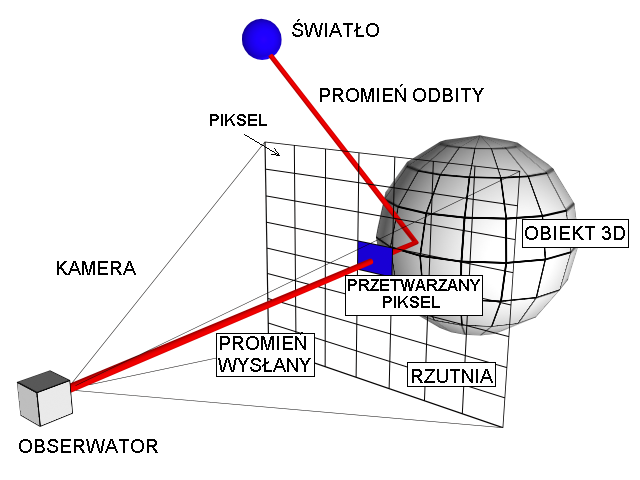
\includegraphics[width=\textwidth]{roz3/img/barwa_pixela.png}
	\caption{Spos�b okre�lania barwy piksela w raytracigu}
	\label{fig:barwa_pixela}
\end{figure}


\begin{figure}[h]
	\centering
		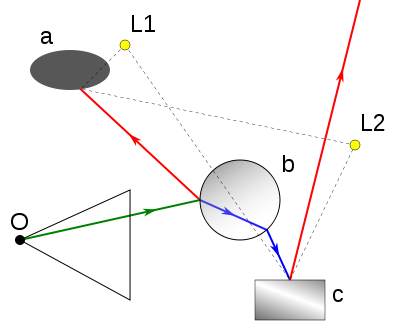
\includegraphics[width=\textwidth]{roz3/img/rekursywny_algorytm.png}
	\caption{Zasada dzia�ania rekursywnego algorytmu ray tracingu}
	\label{fig:rekursywny_algorytm}
\end{figure}


\section{Rekursywna metoda �ledzenia promieni}
\label{sec:chapter3:RekursywnaMetoda}
Przy omawianiu wstecznej metody �ledzenia promieni warto wspomnie� o raytracingu rekursywnym. W zagadnieniu tym bada si� rekurencyjnie promienie odbite zwierciadlane oraz za�amane, kt�re powsta�y z kolizji promieni pierwotnych 
z obiektami na scenie. Tak wi�c �ywotno�� promienia pierwotnego wcale nie ko�czy si� w momencie kolizji z obiektem sceny. To czy z danego promienia pierwotnego wygenerowane zostan� kolejne promienie w bardzo du�ej mierze zale�y od materia�u jakim pokryty jest dany obiekt sceny. Z pomoc� tego rekursywnej metody �ledzenia promieni jeste�my w stanie zasymulowa� obiekty lustrzane oraz obiekty p�przezroczyste. Rekurencja w tej metodzie trwa do osi�gni�cia maksymalnego stopnia zag��bienia. Kolor wynikowy danego pojedynczego Pixela powstaje z sumy kolor�w, obiektu w jaki trafi� promie� pierwotny oraz kolor�w obiekt�w w jakie trafi�y promienie pierwotne. Poni�ej przedstawiony jest pogl�dowy schemat zasady dzia�ania rekursywnej metody �ledzenia promieni: \ref{fig:rekursywny_algorytm}


\section{Przedstawienie algorytmu �ledzenia promieni}
\label{sec:chapter3:PrzedstawienieAlgorytmu}
�ledzenie promieni przez scen� rozpoczyna si� od obserwatora okre�lanego cz�sto jako kamery wyst�puj�cej na scenie. Przez ka�dy pixel ekranu �ledzone s� promienie kt�re poruszaj� si� po scenie. Gdy kt�ry� ze �ledzonych promieni napotka obiekt i zacznie z nim kolidowa�. 





\section{Przyk�ad sz�sty}

Oto przyk�adowy wydruk:
\begin{lstlisting}[language=C,style=outcode]
/* ta funkcja oblicza a+b */
int sum(int a, int b) 
{
	int suma=0;

	suma=a+b;

	return suma;
}
\end{lstlisting}










% ********** Rozdzia� 4 **********
\chapter{NVIDIA CUDA jako znakomita platforma do zr�wnoleglenia oblicze�}
\label{sec:chapter4}


\section{Wst�pny opis}
\label{sec:chapter4:Wstep}
CUDA(Compute Unified Device Architecture) jest do�� now� technologi� wprowadzon� na rynek przez firm� NVIDIA. Technologia ta sw�j pocz�tek mia�a w 2007 roku. Od samego pocz�tku sta�a si� ona wiod�c� technologi� przetwarzania strumieniowego z wykorzystaniem GPU. CUDA jako, �e jest technologi� stworzon� przez firm� NVIDIA, wspierana jest przez uk�ady graficzne w�a�nie tej firmy. Wsparcie dla tej technologii rozpocz�o si� od uk�ad�w graficznych serii GeForce 8, Quadro oraz Tesla. Seria uk�ad�w graficzny Quadro oraz Tesla s� wyspecjalizowanymi uk�adami obliczeniowymi do zastosowa� naukowych. Natomiast serie GeForce mo�na spotka� na co dzie� w komputerach stacjonarnych oraz laptopach. Z pomoc� technologii CUDA jeste�my wstanie uzyska� wielokrotne przy�pieszenie w obliczeniach w stosunku do oblicze� na zwyk�ym procesorze CPU. na ryskunku \ref{fig:processing_flow_cuda} przedstawiony zosta� przyk�adowy schemat przep�ywu oblicze� w CUDA.

\begin{figure}[h]
	\centering
		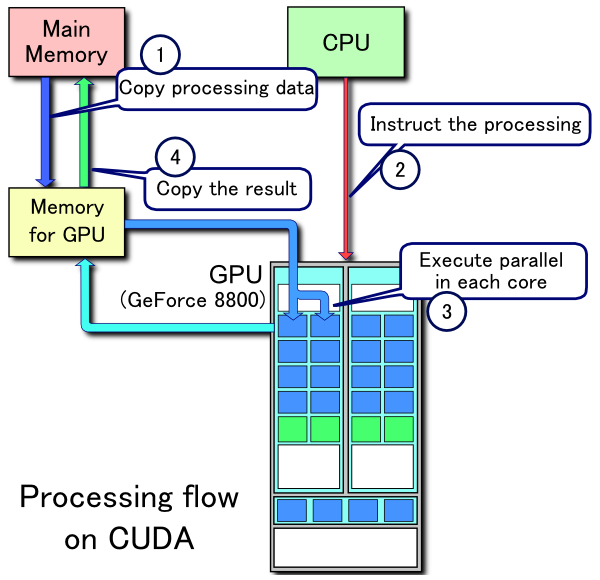
\includegraphics[width=0.5\textwidth]{roz4/img/processing_flow_cuda.png}
	\caption{Przyk�ad przep�ywu przetwarzania w technologii CUDA.}
	\label{fig:processing_flow_cuda}
\end{figure}

\section{Wspierane karty oraz zdolno�� obliczeniowa}
\label{sec:chapter4:Wspierane_karty}
We wst�pnym opisie powiedziane by�o, �e technologia CUDA zapocz�tkowana by�a w uk�adach graficznych serii GeForce, Tesla oraz Quadro. W tabeli \ref{tab:wspierane_karty} przedstawione zosta�o oficjalne wsparcie okre�lonej wersji CUDA w poszczeg�lnych uk�adach graficznych.
\\\\\\\\

\begin{table}[h]
\centering
\begin{tabular}{| p{5cm} | p{2cm} | p{6cm} |}
\hline
Zdolno�� obliczeniowa (wersja) & GPUs & Cards \\
\hline
1.0 & G80 & GeForce 8800GTX/Ultra/GTS, Tesla C/D/S870, FX4/5600, 360M \\ \hline
1.1 & G86, G84, G98, G96, G96b, G94, G94b, G92, G92b & GeForce 8400GS/GT, 8600GT/GTS, 8800GT, 9600GT/GSO, 9800GT/GTX/GX2, GTS 250, GT 120/30, FX 4/570, 3/580, 17/18/3700, 4700x2, 1xxM, 32/370M, 3/5/770M, 16/17/27/28/36/37/3800M, NVS420/50 \\ \hline
1.2 & GT218, GT216, GT215 & GeForce 210, GT 220/40, FX380 LP, 1800M, 370/380M, NVS 2/3100M \\ \hline
1.3 & GT200, GT200b & GTX 260/75/80/85, 295, Tesla C/M1060, S1070, CX, FX 3/4/5800 \\ \hline
2.0 & GF100, GF110 & GTX 465, 470/80, Tesla C2050/70, S/M2050/70, Quadro 600,4/5/6000, Plex7000, 500M, GTX570, GTX580 \\ \hline
2.1 & GF108, GF106, GF104 & GT 420/30/40, GTS 450, GTX 460 \\ \hline
\end{tabular}
\caption{Zestawienie kart graficznych oficjalnie wspieraj�cych technologi� CUDA.}
\label{tab:wspierane_karty}
\end{table}

Kolejn� wa�n� rzecz� wyr�niaj�ca karty graficzne jest ich zdolno�� obliczeniowa (ang. compute capability). Identyfikuje ona mo�liwo�ci obliczeniowe danej karty graficznej w odniesieniu do technologii NVIDIA CUDA.  W tabeli \ref{tab:porownanie_zdolnosci} przedstawione zosta�y mo�liwo�ci kart graficznych w zale�no�ci od profilu CUDA.


\begin{table}[h]
\centering
\begin{tabular}{ | p{6cm} | p{1cm} | p{1cm} |  p{1cm} |  p{1cm} |}
\hline
Zdolno�� obliczeniowa & 1.0 & 1.1 & 1.2 & 1.3 \\
\hline
Funkcje atomowe w pami�ci globalnej & - & \checkmark & \checkmark & \checkmark \\ \hline
Funkcje atomowe w pami�ci wsp�dzielonej & - & - & \checkmark & \checkmark \\ \hline
Ilo�� rejestr�w na multiprocesor & 8192 & 8192 & 16384 & 16384 \\ \hline
Maksymalna liczba warp�w na multiprocesor & 24 & 24 & 32 & 32 \\ \hline
Maksymalna liczba aktywnych w�tk�w na multiprocesor & 768 & 768 & 1024 & 1024 \\ \hline
Podw�jna precyzja & - & - & - & \checkmark \\ \hline
\end{tabular}
\caption{Por�wnanie zdolno�ci obliczeniowych kart graficznych wspieraj�cych NVIDIA CUDA.}
\label{tab:porownanie_zdolnosci}
\end{table}

\section{Architektura}
\label{sec:chapter4:architektura}
Karty graficzne GPU znacznie r�ni� si� wydajno�ci� od zwyk�ych procesor�w CPU. R�nica w wydajno�ci wynika g��wnie z faktu, i� procesory graficzne specjalizuj� si� w r�wnoleg�ych, wysoce intensywnych obliczeniach. Karty graficzne sk�adaj� si� z wi�kszej liczby tranzystor�w kt�re s� odpowiedzialne za obliczenia na danych. Nie posiadaj� natomiast takiej kontroli przep�ywu instrukcji oraz jednostek odpowiedzialnych za buforowanie danych jak procesory komputerowe CPU.  Uk�ady graficzne wspieraj�ce technologi� CUDA zbudowane z multiprocesor�w strumieniowych (ang. stream multiprocessor). R�ne modele kart graficznych firmy NVIDIA posiadaj� r�n� liczne multiprocesor�w, co przek�ada si� tak�e na wydajno�� i zdolnos� obliczeniow� danej architektury. Na rysunku \ref{fig:multiprocesor}
Przedstawiona jest przyk�adowa budowa takiego w�a�nie multiprocesora.

\begin{figure}[h]
	\centering
		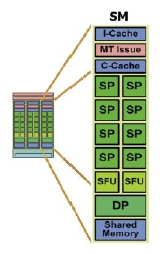
\includegraphics[width=0.5\textwidth]{roz4/img/multiprocesor.jpg}
	\caption{Przyk�adowy schemat multiprocesora strumieniowego.}
	\label{fig:multiprocesor}
\end{figure}


Ka�dy z multiprocesor�w sk�ada si� z: (napisac z kad to wziete!!!!!)
\begin{itemize}  
  \item I-Cache - bufor instrukcji  
  \item MT Issue - jednostka kt�ra rozdziela zadania dla SP i SFU
  \item C-Cache -bufor sta�ych (ang. constant memory) o wielko�ci 8KB, kt�ry przyspiesza odczyt z obszaru pami�ci sta�ej 
  \item 8 x SP - 8 jednostek obliczeniowych tzw stream processors, kt�re wykonuj� wi�kszo�� oblicze� pojedynczej precyzji (ka�dy zawiera w�asne 32-bitowe rejestry)
  \item 2 x SFU  - jednostki specjalne (ang. special function units). Zadaniem ich jest obliczanie funkcji przest�pnych, np. trygonometrycznych, wyk�adniczych i logarytmicznych, czy interpolacja parametr�w. 
  \item DP -procesor, kt�ry wykonuje obliczenia podw�jnej precyzji
  \item SM - pami�� wsp�dzielona (ang. shared memory) o wielko�ci  16KB.
\end{itemize}  

\section{Rodzaje pami�ci w architekturze CUDA}
\label{sec:chapter4:pamieci}
\begin{itemize} 
\item Pami�� globalna (ang. global memory) - Ta pami�� jest dost�pna dla wszystkich w�tk�w. Nie jest pami�ci� buforowan�. Dost�p do niej trwa od oko�o 400 do 600 cykli. Pami�� ta s�u�y przede wszystkim do zapisuj wynik�w dzia�a� programu obliczeniowego.

\item Pami�� lokalna (ang. local memory) - Ma taki sam czas dost�pu jak pami�� globalna (400-600 cykli). Nie jest tak�e pami�ci� buforowan�. Jest ona zdefiniowana dla danego w�tku. Ka�dy w�tek CUDA posiada w�asn� pami�� lokaln�. Zajmuje si� ona przechowywaniem bardzo du�ych struktur danych. Pami�� ta jest najcz�ciej u�ywana gdy obliczenia danego w�tku nie mog� by� w ca�o�ci wykonane na dost�pnych rejestrach procesora graficznego.

\item Pami�� wsp�dzielona (ang. shared memory) - Jest to bardzo szybki rodzaj pami�ci, dor�wnuj�cy szybko�ci rejestr�w procesora graficznego. Przy pomocy tej pami�ci, w�tki przydzielone do jednego bloku s� wstanie si� ze sob� komunikowa�. Nale�y jednak obchodzi� si� ostro�nie z tym rodzajem pami�ci, gdy� mog� powsta� Momoty w kt�rych w�tki w jednym bloku b�d� chcia�y jednocze�nie zapisywa� i odczytywa� z tej pami�ci. Wyst�powanie takich konflikt�w w odczycie i zapisie powoduje du�e op�nienia.

\item Pami�� sta�a (ang. const memory) - Ta pami�� w odr�nieniu do powy�szych rodzaj�w pami�ci, jest buforowan� pami�ci� tylko do odczytu. Gdy potrzebne dane znajduj� si� aktualnie w buforze dost�p do nich jest bardzo szybki. Czas dost�pu ro�nie gdy danych nie ma w buforze i musz� by� doczytane z pami�ci karty.

\item Pami�� Tekstur (ang. texture memory) - Jest pami�ci� podobn� do pami�ci sta�ej gdy� udost�pnia tylko odczyt danych. Jest tak�e pami�ci� buforowan�. W pami�ci tej bufor danych zosta� zoptymalizowany pod k�tek odczytu danych z bliskich sobie adres�w. Najkorzystniejsz� sytuacj� jest gdy w�tki dla danego warpa (grupa 32 w�tk�w zarz�dzanych przez pojedynczy multiprocesor) odczytuj� adresy, kt�re znajduj� si� blisko siebie. CUDA w swojej implementacji udost�pnia mo�liwo�� pos�ugiwania si� teksturami 1D,2D,3D.

\item Rejestry - Jest to najszybszy rodzaj pami�ci. Dost�p do niego nie powoduje �adnych dodatkowych op�nie�, chyba �e pr�bujemy odczyta� z rejestru do kt�rego dopiero co zosta�o co� zapisane. Ka�dy multiprocesor w urz�dzeniu CUDA posiada 8192 lub 16384 rejestr�w 32-bitowych. Zale�y to od wersji(zdolno�ci obliczeniowej) danego urz�dzenia. W celu unikni�cia powy�szych konflikt�w ilo�� w�tk�w na pojedynczy multiprocesor ustawia si� jako wielokrotno�� liczby 64. NAPISAC Z KAD TO WIEM!!!!!!!!!!!!!1
\end{itemize} 


Na obrazku \ref{fig:pamiec} poni�ej przedstawiony zosta� pogl�dowy schemat pami�ci w architekturze CUDA.
\begin{figure}[h]
	\centering
		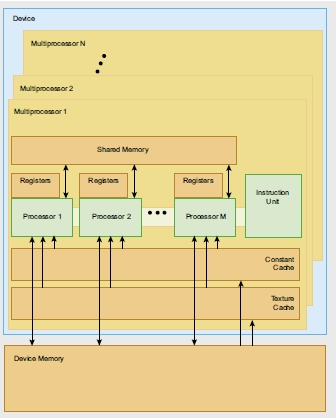
\includegraphics[width=0.5\textwidth]{roz4/img/pamiec.jpg}
	\caption{Schemat pami�ci.}
	\label{fig:pamiec}
\end{figure}



\section{Przyk�adowy program pod architektur� CUDA}
\label{sec:chapter4:kod}
Poni�ej przedstawiony zosta� przyk�ad programu napisanego w j�zyku C dla architektury CUDA. Program ten uruchamiany jest na wielu w�tkach karty graficznej, ka�dy z tych w�tk�w niezale�nie wpisuj� do tablicy swoje ID.
Wa�n� informacj� przy pisaniu kodu dla architektury CUDA jest to, �e funkcje uruchamiane przez w�tki maj� specjalne oznaczenia:
\begin{itemize} 
\item global - funkcje tak� wywo�a� mo�na tylko z CPU, a wykonuje si� ona na GPU
\item host - funkcjawykonuje si� i mo�e by� wywo�ana tylko z kodu wykonywanego na CPU
\item device - funkcja wykonuje si� i mo�e by� wywo�ana tylko z kodu wykonywanego na GPU
\end{itemize} 

Nale�y tak�e pami�ta� �e funkcje dla w�tk�w CUDA musz� zawsze zwracac wartosc \textit void.

\begin{lstlisting}[language=C,style=outcode]
#include <stdlib.h>
#include <cuda_runtime.h>
#include <cutil.h>

// definicja funkcji kt�ra b�dzie uruchamiana 
// r�wnolegle na w�tkach CUDA
__global__ void testFunction(int *data)
{
	// obliczamy index tablicy a zarazem w�tku
	int id = blockIdx.x * blockDim.x + threadIdx.x;
	// Zaposujemy do tablicy ID w�tku
	data[id] = id;
}

// W funkcji main wywo�ujemy powy�sz� funkcje
// dla w�tk�w CUDA
int main()
{
	// Na poczatku nale�ey zainicjowa� urz�dzenie CUDA
	cudaSetDevice(0);

	// alokujemy pamie� na karcie graficznej
	int *tablica;
	cudaMalloc((void**)&tablica, sizeof(int) * ARRAY_SIZE); 

	// Ustalamy wielkosc bloku i karty
	dim3 dimBlock(BLOCK_SIZE, 1); 
	dim3 dimGrid(ARRAY_SIZE / dimBlock.x, 1);

	// wywo�ujemy nasz� funkcj� obliczeniow�
	testFunction<<<dimGrid, dimBlock>>>(tablica);

	// Tworzymy tablice w pamieci ram i kopujemy
	// dane z karty graficznej do pamieci ram.
	int *tablica2 = (int*)malloc(sizeof(int) * ARRAY_SIZE);
	cudaMemcpy(tablica, tablica2, sizeof(int) * ARRAY_SIZE,
	cudaMemcpyDeviceToHost);

	return 0;
}
\end{lstlisting}

Jak widzimy na powy�szym listingu kodu gdy wywo�ujemy funkcj� CUDA okre�lamy na ilu w�tkach ma si� ona uruchomi� i w jakie grupy maj� by� one pogrupowane.
Na rysunku JAKIS RYSSSSSSSSSSSSSSSss przedstawiony zosta� schemat pokazuj�cy jak mog� wygl�da� u�ywane w�tki w ca�ej kgracie, pogrupowane w odpowiednie bloki.
Podczas programowania na karty graficzne CUDA nale�y pami�ta� o r�nych dost�pnych rodzajach pami�ci i wybra� t� naj�a�ciwsz�. Je�li nie przemy�limy dobrze problemu jaki sobie za�o�yli�my rozwi�za� przy pomocy technologii CUDA, mo�e si� zda�y�, �e nasze rozwi�zanie b�dzie dzia�a�o gorej ni� na procesorze CPU. Nale�y tak�e poinformowa� o tym, �e brak jest narz�dzi, kt�re wspomaga�y by �ledzenie przep�ywu wykonywania programu tzw debugowanie. Z tym problemem borykaja si� wszystkie technologie zwiazane z GPGPU( obliczenia przeprowadzane na kartach graficznych ).

% ********** Rozdzia� 5 **********
\chapter{Om�wienie aplikacji testowej}
\label{sec:chapter5}


\section{Za�o�enia}
\label{sec:chapter5:zalozenia}
Na potrzeby niniejszej pracy zosta�o opracowane autorskie rozwi�zanie uniwersalnego wstecznego raytracera dzia�aj�cego zar�wno na procesorze CPU jak i r�wnie� na ko-procesorach graficznych GPU firmy NVIDIA. Aplikacja testowa jest wstanie generowa� wynikowe obrazy scen 3D sk�adaj�cych si� z kul, prostopad�o�cian�w oraz p�aszczyzn. Na ka�dy z element�w sceny jest mo�liwo�� na�o�enia dowolnej tekstury oraz doboru odpowiednich parametr�w materia�u. Dodatkowo na scenie mo�liwe jest umieszczanie �wiate� punktowych. Aplikacja sama w sobie jest benchmarkiem, kt�ry potrafi przetestowa� zadan� liczb� scen 3D na komputerze u�ytkownika. Zebrane wyniki z oblicze� jest wstanie przes�a� na wybrany adres e-mail (w tym przypadku za zgod� u�ytkownika do developera). Aplikacja przy generowaniu obrazu sceny 3D bierze pod uwagi r�ne w�a�ciwo�ci materia�u danego obiektu. Docelowo generowane s� takie efekty jak: o�wietlenie, odblask, cienie, wielokrotne odbicia i za�amania, tekstury. Przy u�yciu materia��w o r�nych parametrach jeste�my wstanie uzyska� bardzo ciekawie wygl�daj�ce obiekty np: lustro, szk�o, metale i wiele innych.


\section{Implementacja}
\label{sec:chapter5:implementacja}
Aplikacja testowa zosta�a napisana w j�zyku C++, wykorzystuj�c biblioteki standardowe pochodz�ce z j�zyka C. Wersja �ledzenia promieni przy u�yciu technologii CUDA zosta�a napisana w tzw. "C for CUDA". Dodatkowo do wy�wietlania wynikowych obraz�w u�yta zosta�a biblioteka Microsoft DirectX 9.0. Wersja �ledzenia promieni dzia�aj�ca na CPU jest tak�e zr�wnoleglona na wszystkie procesory znajduj�ce si� w danym komputerze. U�yta do tego zosta�a bilioteka open source "OpenMP". Program przeznaczony jest do uruchamiania na systemach z rodziny Windows. Aplikacj� testow� mo�na nazwa� swoistym benchmarkiem. Dzia�anie jej sk�ada si� z 5 wa�nych punkt�w:
\begin{itemize}  
\item wczytywanie scen do testow
\item testowanie zadanych scen na procesorze CPU.
\item testowanie zadanych scen na karcie graficznej GPU.
\item zapisywanie wynikowych obraz�w scen na dysk u�ytkownika
\item zebranie informacji o testowanych scenach i wys�anie ich na mail developera.
\end{itemize}

\textbf{Przebieg dzia�ania:}\\
Aplikacja na samym pocz�tku wczytuje plik benchamarku z rozszerzeniem *.rtb. Plik ten zawiera w sobie spis scen (pliki *.rtm) kt�re maj� by� przetestowane przez raytracer. Nast�pnie rozpoczyna si� testowanie zadanych scen na procesorze CPU.  Gdy wszystkie sceny zostan� przetestowane na procesorze, rozpoczyta si� raytracing na karcie graficznej z u�yciem CUDA. Na koniec gdy ju� wszystkie sceny zosta�y wygenerowane przy u�yciu CPU oraz GPU, wynikowe obrazy generowane przez raytracer zapisywane s� na dysku u�ytkownika. Zebrane informacje z profilowania ka�dej ze scen zostaj� zapisane do pliku oraz wys�ane na adres e-mail developera.
\\\\
\textbf{Statystyki zwi�zane z kodem aplikacji testowej:}\\
\begin{itemize} 
\item 61 plik�w kodu
\item 9386 linii kodu
\item 272697 bajt�w kodu
\end{itemize}
\clearpage

Poni�ej zaprezentowany zosta� diagram najwa�niejszych klas dla aplikacji testowej raytracera:\\

\begin{figure}[h]
	\centering
		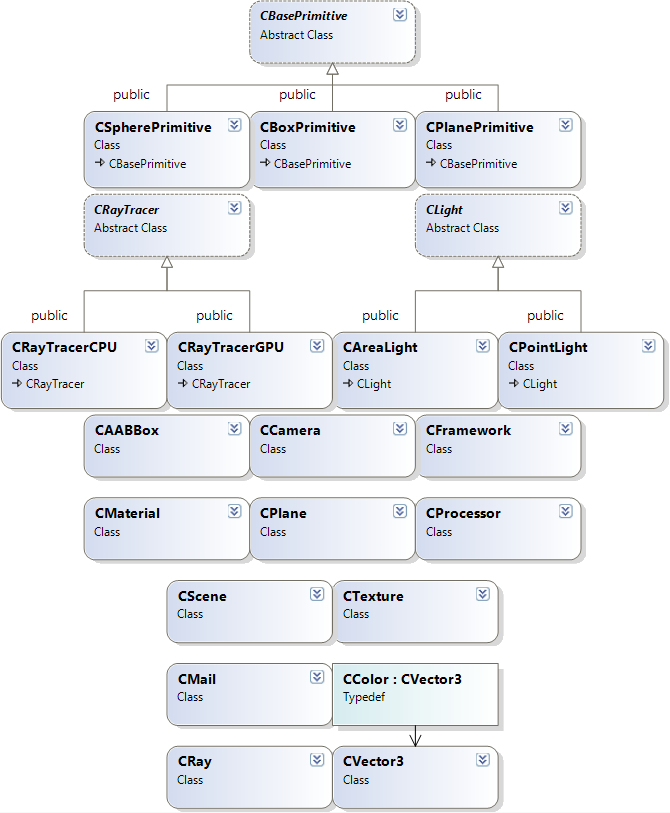
\includegraphics[width=\textwidth]{roz5/img/class_diagram.png}
	\caption{Diagram klas aplikacji testowej}
	\label{fig:class_diagram}
\end{figure}


\section{Zestaw test�w}
\label{sec:chapter5:zestaw_testow}
By wykaza� przy�pieszenie pomi�dzy �ledzeniem promieni na procesorze CPU a kart� graficzn� GPU przygotowany zosta� zestaw 9 scen testowych. Testowana jest wydajno�� generowania scen o r�nej budowie i wyst�puj�cych na niej prymitywach. W scenach tych testowanych jest wiele parametr�w takich jak:
\begin{itemize} 
\item Odbicia promieni od obiekt�w na scenie
\item Za�amania promieni w obiektach na scenie
\item Teksturowanie obiekt�w sceny
\item R�na ilo�� �wiate� punktowych na scenie
\item Rodzaj oraz ilo�� prymityw�w wy�wietlanych na scenie
\item Jako�� generowanego obraz (super sampling)
\item Rozdzielczo�� generowanego obrazu
\end{itemize} 


\section{Przyk�ady wygenerowanych obraz�w}
\label{sec:chapter5:wygenerowane_obrazy}
W rozdziale tym przedstawione zosta�y wyniki generowania scen przez aplikacje testow�. Ka�da z tych scen by�a generowana na procesorze CPU oraz na karcie graficznej GPU.
\begin{figure}[h]
	\centering
		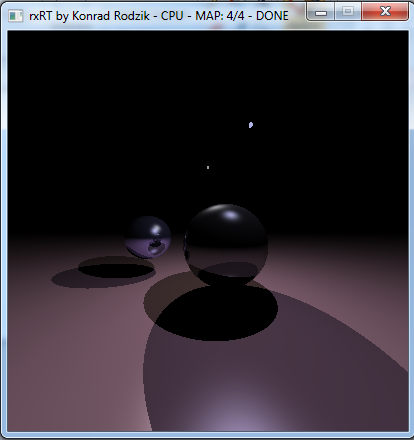
\includegraphics[width=0.7\textwidth]{roz5/img/rt1.png}
	\caption{Przyk�adowa wygenerowana scena 1.}
	\label{fig:rt1}
\end{figure}
\begin{figure}[h]
	\centering
		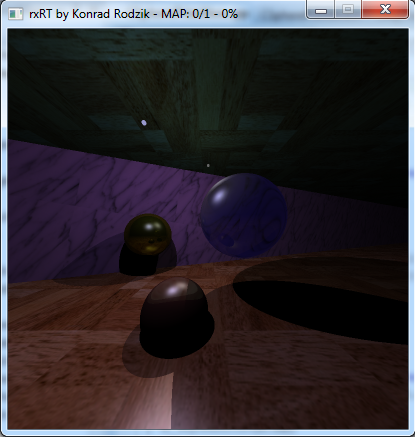
\includegraphics[width=0.6\textwidth]{roz5/img/rt2.png}
	\caption{Przyk�adowa wygenerowana scena 2.}
	\label{fig:rt2}
\end{figure}
\begin{figure}[h]
	\centering
		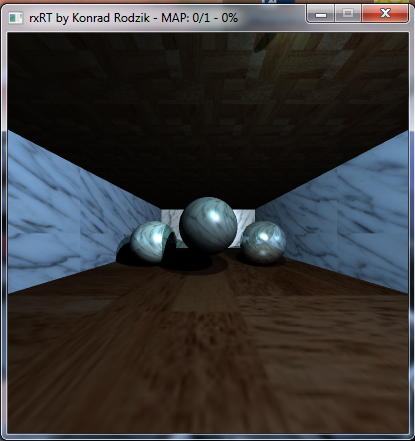
\includegraphics[width=0.6\textwidth]{roz5/img/rt3.png}
	\caption{Przyk�adowa wygenerowana scena 3.}
	\label{fig:rt3}
\end{figure}

% ********** Rozdzia� 6 **********
\chapter{Por�wnanie wydajno�ci Raytracera dzia�aj�cego na CPU oraz na GPU}
\label{sec:chapter6}
Tutaj przedstawi� wszelkie wyniki generowania obraz�w ze scen oraz wszelkie warto�ci czasowe im odpowiadaj�ce.  Por�wnanie wynik�w dla raytracingu CPU vs GPU. Z ka�dych wynikowych danych bada� przeprowadzonych na r�nych konfiguracjach sprz�towych wygenerowany zostanie wykres przedstawiaj�cy r�nice czasowe w generowaniu scen a tym samym przyspieszenie wstecznego raytracingu jakie uda�o si� uzyska�.
Zak�adam wst�pnie testy 10 scen. Na ka�dej z nich r�na konfiguracja obiekt�w oraz materia��w im nadanych. Chce pokaza� jakie w�a�ciwo�ci materia��w i jaka ilo�� prymityw�w oraz ich rodzaj�w wp�ywa na zmniejszanie/zwi�kszanie wydajno�ci raytracingu.


\section{Test1 - TMP TEXT}
\label{sec:chapter6:test1}

\section{Test2 - TMP TEXT}
\label{sec:chapter6:test2}

\section{Test3 - TMP TEXT}
\label{sec:chapter6:test3}

\section{Test4 - TMP TEXT}
\label{sec:chapter6:test4}

\section{Test5 - TMP TEXT}
\label{sec:chapter6:test5}

\section{Test6 - TMP TEXT}
\label{sec:chapter6:test6}

\section{Test7 - TMP TEXT}
\label{sec:chapter6:test7}

\section{Test8 - TMP TEXT}
\label{sec:chapter6:test8}

\section{Test9 - TMP TEXT}
\label{sec:chapter6:test9}

\section{Test10 - TMP TEXT}
\label{sec:chapter6:test10}

\section{Podsumowanie test�w}
\label{sec:chapter6:podsumowanie}

% ********** Rozdzia� 7 **********
\chapter{Podsumowanie i wnioski}
\label{sec:chapter7}
Podsumuje jasna dla wszystkich rzecz, �e obliczenia na kartach graficznych przewy�szaj� wydajno�ci� obliczenia na zwyk�ych wielordzeniowych procesorach komputerowych. Dodatkowo opisze moje przemy�lenia i wnioski kt�re objawi�y mi si� podczas pisania uniwersalnej aplikacji wstecznego raytracingu.
Na koniec opowiem troch� o tym co uda�o si� zrobi�, osi�gn�� a czego nie i w jaki spos�b chcia�bym dalej rozwija� prace nad raytracingiem.



% *************** Bibliography ***************
\nocite{*}
\bibliographystyle{plain}
{\small\bibliography{mobiStopowicz}}

% *************** Appendixes ***************
%\appendix
%\appendixpage*
%% ********** Dodatek 1 **********
\chapter{Terminologia stosowana w pracy}
\label{sec:appendix1}


\begin{itemize} 
\item CUDA - Technologia stworzona przez firm� NVIDIA w 2007 roku. Umo�liwia r�wnoleg�e obliczenia na mikroprocesorach karty graficznej.
\item Benchmark - Aplikacja testowa, kt�ra profiluje wydajno�� i zbiera informacje.
\item Warp - blok w�tk�w przydzielony na multiprocesor.
\item DirectX - technologia graficzna firmy Microsoft. Umo�liwia wy�wietlanie wysokiej jako�ci grafiki 2D/3D.
\item Aliasing - Zdeformowany, o z�ej jako�ci obraz kt�ry powstaje podczas rastaryzacji, powodowany przez zbyt ma�a cz�stotliwo�� pr�bkowania na pojedy�czy piksel obrazu. Przeciwdzia�a si� temu efektowi poprzez antyaliasing oraz w raytracingu poprzez super-sampling.
\item Super-sampling - spos�b na zwi�kszenie jako�ci generowanych scen. Polega na �ledzeniu wielu promieni �wietlnych na pojedy�czy piksel generowanego obrazu.
\end{itemize} 

% ********** Koniec dodatku **********


% *************** Back matter ***************
\backmatter
% *************** Back matter ***************

% *******************************************************************************************
% W tym miejscu mo�esz wy��czy� tworzenie spisu symboli, spisu ilustracji, spisu tre�ci
% Mo�esz tak�e wy��czy� tworzenie skorowidza
% *******************************************************************************************

\backmatter

%\clearpage
%\lstlistoflistings

\clearpage
\listoffigures

\clearpage
\listoftables


\footnotesize
\printindex

% *************** Koniec back matter ***************


\end{document}
